\chapter{Background and Related Work Analysis}\label{bg}
In this chapter we provide reader with the base knowledge in field of Optimization Problems and the process of their solving.
The reader who is an expert in field of Optimization and Search Problems could find this chapter as an obvious discussion of well-known facts. If the notions of \textit{Parameter Tuning} and \textit{Parameter Control} seems like two different names for one thing, we encourage you to read this chapter carefully.
We highly recommend for everyone to refresh the knowledge of sections topics and examine the examples of Hyper-Heuristics in \ref{bg: hh examples} and Systems for parameter tuning in \ref{bg: parameter tuning expamples} since we use them later in concept implementation.

% TODO: finalize intro to chapter
% add brief outline of lieterature review

\section{Optimization Problems and their Solvers}\label{bg:opt problems and solvers}


\subsection{Optimization Problems}\label{BG: subsection OPs}
%https://www.solver.com/problem-types
% need to add some kind of catchy intro, here or in previous parts of this section.
While the Search Problem (SP) defines the process of finding a possible Solution for the Computation Problem, an Optimization Problem (OP) is the special case of the SP, focused on the process of finding the \emph{best possible} Solution for Computation Problem~\cite{goldreich2010p}. 


In this thesis we focus on the Optimization Problems — a special case of the Search Problems.


A lot of conducted studies in this field have tried to formalize the concept of OP, but the underlying notion such a vast that it is almost impossible to exclude the application domain from the definition. The description of every possible Optimization Problem and all approaches for solving it are out of the scope of this thesis. However, a birds-eye view should be presented in order to make sure that reader is familiar with all notions used through this thesis. 


In \cite{biegler2004retrospective,figueira2014hybrid,amaran2016simulation} authors distinguished OP characteristics that overlap through each of these works and those we would like to start from them.


First, let us define the subject of the Optimization. In general, it could be imagined as the Target System (TS) displayed on picture \ref{bg:pic:Target System}. Analytically it could be represented as the function $Y = f(X)$. Informally it accepts the information with its \textit{inputs} \textbf{X} sometimes also called variables or parameters, performs a \textit{Task} and produces the result on its \textit{outputs} \textbf{Y}.

\svgpath{{graphics/Background/}}
\begin{figure}
	\centering
	\includesvg[width=0.5\textwidth]{TargetSystem}
	\caption{Target System}
	\label{bg:pic:Target System}
\end{figure}

Pair of $X$ and respective $Y$ form a \textit{Solution} for Computation Problem.
All possible inputs $X$ form a \textit{Search Space}, while all outcomes $Y$ form an \textit{Objective Space}.
The Solution could also be characterized by the \textit{objective} value(s) — a quantitative measure of TS performance that we minimize or maximize. 
We could obtain those value(s) directly by reading the $Y$, or indirectly for instance, noting the time TS took to produce the output $Y$ for given $X$. 
The Solution objective value(s) form object(s) of Optimization. 
For the sake of simplicity we here use $Y$, \textit{outputs}, \textit{objectives} and $X$, variables, \textbf{parameters(?)}% will decide later
 interchangeably.


Next, let us highlight the Target System characteristics.
Among mentioned in \cite{biegler2004retrospective,figueira2014hybrid,amaran2016simulation} we found those the most important:
\begin{itemize}[itemsep=8pt]
	\item \textbf{Input data types} of $X$ is a crucial characteristic. The variables could be either \textit{discrete} where representatives are binary strings, integer-ordered or categorical data, % One could apply mixed integer linear (nonlinear) programming here (MILP, MINLP) \cite{biegler2004retrospective}.
	\textit{continuous} where variables are usually a range of real numbers, or \textit{mixed} as the mixture of previous two cases.

	\item \textbf{Constrains} are functional dependencies that describe the relationships among inputs and defile the allowable values for them.

	\item \textbf{Amount of knowledge} TS exposes about the dependencies between $X \rightarrow Y$ or objective values. With respect to this knowledge, the Optimization could be \textit{White Box} — the TS exposes it internals fully, so it is even possible to derive the algebraic model of TS.
	%\textit{Gray Box} - the amount of exposed knowledge is significant, but not enough to build the algebraic model.
	\textit{Black Box} — the exposed knowledge is mostly negligible.
	%In this case the Derivative Free Optimization approaches (such as Surrogate Optimization, different Meta-|Hybrid-|Hyper-Heuristics)  are applicable.

	%\paragraph{Dependency types} could be  The inputs to outputs dependencies the of Target System could also be distinguished form perspective of linearity \cite{biegler2004retrospective,figueira2014hybrid}.
	%\textit{Linear dependencies} reveal the Linear Programming Optimization approaches, while with \textbf{Nonlinear dependencies} one should consider Nonlinear Programming.

	\item \textbf{Dependencies randomness} One of possible challenges, while obtaining the knowledge about TS is uncertainty of output. Ideal case is the \textit{deterministic} dependency between $X$ and $Y$, however in most of real-world challenges engineers tackle with the \textit{stochastic} systems whose output is affected by random processes. 

	\item \textbf{Cost of evaluation} is the amount of resources (computational, time, money, etc.) TS will spend to obtain the result for particular input. It varies from very cheap if the TS is a simple algebraic formula and Task is to evaluate it, to very expensive if the TS is a complex Neuron Network and the Task is to train it on data.

	\item \textbf{Number of objectives} could be either \textit{Single}, or \textit{Multiple}. According to the number of objectives, the result of optimization will be either single Solution, or set of non-dominated (Pareto-optimal) Solutions \cite{deb2014multi}.

\end{itemize}


Combining different characteristic, one could obtain broad range of Optimization Problem types.


In this thesis we tackle such a real life problems as bin packing, job-shop scheduling or vehicle routing.
The mentioned above problems has been shown to impose $NP-complete$ (meaning that they are both $NP$ and $NP-hard$) computational complexity \cite{garey1979computers}.


As an example, let's grasp these characteristics for Traveling Salesman Problem (TSP) \cite{applegate2006traveling} — an instance of vehicle routing problem and one of the most studied combinatorial OP, yet still remaining one of the most challenging (here we consider deterministic, symmetric TSP).
The informal definition of TSP is as follows: 'Given a set of cities and the distances between each of them, what is the shortest path to visit each city once and return to the origin city?'.
The input data (path) is a vector of city indexes, and those the type is a non-negative integers \textit{0, 1, 2...}.
There are two constrains on path: it should contain only unique indexes (those, each city will be visited only once) and it should start and end from the same city. 
The TSP distance (or cost) matrix here plays role of Target System, clearly that this TS exposes all internal knowledge and those it is the white box.
Since the cost matrix is fixed and not changing, the TS is considered to be deterministic, cost for two identical paths are always the same (although there exist Dynamic TSP where the cost matrix changes while computing the path cost to reflect a real-time traffic information updates while traveling \cite{cheong2011dynamic}).
It is extremely cheap to compute a cost for given path using cost matrix, those overall Solution evaluation in this TS is cheap.
Since we are optimizing only the route distance, it is a Single objective OP.


\subsection{Optimization Problem Solvers}\label{BG: subsection OP Solvers}
Any Optimization Problem could be solved by an exhaustive search. 
But when the problem size significantly increase, the amount of time needed for an exhaustive search becomes infeasible and in most cases even relatively small problem instances could not be solved by an enumeration.

Here different techniques come into play, but the provided by Target System characteristics of Optimization Problem could restrict and sometimes strictly define the applicable approach.
For instance, imagine you have white box deterministic TS with discrete constrained input data and cheap evaluation. The OP in this case could be described using Integer Linear Programming \todoy{ref} approaches, or heuristics \todoy{ref}. If this TS turned out to be a black box, the ILP approaches are not applicable and one should consider using heuristics \cite{biegler2004retrospective}.


Again, there exist a lot of different facets for OP Solvers classification, however they are a subject of surveying works. Here as the point of interest we decided to highlight two of them.

From the perspective of solution quality:
\begin{itemize}
	\item \textbf{Exact} Solvers are those algorithms that always provide an optimal Solution for OP.
	\item \textbf{Approximate} Solvers produce a sub-optimal output with guarantee in quality (some order of distance to the optimal solution).
	\item \textbf{Heuristics} Solvers do not give any worst-case guarantee for the final result quality.
\end{itemize}

From the perspective of solution availability:
\begin{itemize}
	\item Algorithms that expose the Solution \textbf{at the end} of their run.
	\item In opposite, \textbf{anytime} algorithms designed to improve the solution quality step-by-step while solving the OP and those, intermediate results are naturally accessible. 
\end{itemize}

Each if this algorithm families has own advantages and disadvantages in comparison to other, and if the property of solution availability is clear, the solution quality faced require more detailed description.

\subsubsection{Solution Quality Classes}
\paragraph{Exact Solvers.}
As we stated previously, the exact algorithms are those which always solve an OP to optimality.

For some OP it is possible to develop an algorithm that is much faster than exhaustive search — it runs in super-polynomial time providing an optimal solution. As it stated in \cite{woeginger2003exact}, if the common belief $P \ne NP$ is true, those super-polynomial time algorithms are the best we can hope to get when dealing with an NP-complete problem.

By the definition in \cite{fomin2013exact}, the objective of an exact algorithm is to perform better (in terms of running time) than exhaustive search.
In both works \cite{woeginger2003exact} author had enumerated the main techniques for exact algorithms designing each of which enhance this 'better' independently.
A brief explanation of them will help to refresh the knowledge.

\begin{itemize}
	\item \textbf{Branching and bounding} techniques when applied to origin problem, split the search space of all possible solutions (e.g. exhaustive search space) to a set of smaller sub-spaces (more formally, branching the search tree into subtrees). This is done with an intent to later prove that some sub-spaces never lead to an optimal solution and those could be ignored in order to speed-up the search.
	
	\item \textbf{Dynamic programming across the Subsets} techniques in some sort could be combined with the mentioned above branching techniques. After forming the Search Space subsets (branches), the dynamic programming attempts to derive solutions for smaller subsets and combine them into solutions for lager subsets unless finally derive a solution for original search space.
	
	\item \textbf{Problem preprocessing} could be applied as an initial phase of the solving process. This technique is dependable upon the underlying OP, but when applied properly, significantly reduce the running time. A toy example from \cite{woeginger2003exact} elegantly illustrate this technique: imagine problem of finding a pair of two integers $x_i$ and $y_i$ that sum up to integer $S$ in $X_k$ and $Y_k$ sets of unique numbers ($k$ here denotes the size of a set). The exhaustive search will enumerate all $x-y$ pairs in $O(k^2)$ time. But one could first preprocess the data by sorting it, after that use bisection search repeatedly in this sorted array and search for $k$ values $S - y_i$, the overall time complexity becomes $O(k\log(k))$.
\end{itemize}


\paragraph{Approximate Solvers.} When the OP cannot be solved to optimal in polynomial time, people start thinking in alternative solutions and mostly relax their requirements. Approximate algorithms are representatives of the theoretical computer science field that have been created in order to tackle the computationally difficult white box OP. %In words of Garey and Johnson it means "I can't find an efficient (polynomial time) algorithm, but neither can all of these famous people."
%If the widely believed conjecture $P \ne NP$ is true, a wide range of OPs (ILP) are $NP-hard$ and cannot be solved with exact solvers in polynomial time, those require relaxation either in efficiency or quality of optimization.


In contradistinction to exact, approximate algorithms relax the quality requirements and solve an OP effectively with the provable assurances on the result distance from an optimal solution \cite{williamson2011design}. The worst case results quality guarantee is crucial in design of approximation algorithms and involves mathematical proofs. 

One may ask a question ``How do these algorithms guarantee on quality, if the optimal solution is unknown ahead?'' Certainly it sounds contradictive since knowing the optimal solution cancels an optimization problem itself. The answer to this question highlights a key technique in the design of approximation algorithms.

In \cite{williamson2011design} authors stated several techniques of an approximate solvers design. The \textbf{Linear Programming} relaxation plays a central role in approximate solvers. It is well known that solving the ILP is $NP-hard$ problem, however it could be relaxed to polynomial-time solvable LP. %Those, one of techniques is relaxation of ILP to LP. An optimal solution for LP will have value $S_LP \le S_IP = OPT$ (for the minimization case). Here we could derive a lower bound for the original minimization or upper bound for maximization problem. 
Later fractional solution for the LP should be rounded to obtain a feasible solution for the ILP. % that is within a cerain factor $f$ the value of the LP $S_LP$. Thus, the ILP solution will cost no more than $f * OPT$.
Different rounding strategies define separate technique for approximate solvers \cite{williamson2011design}: 
\begin{itemize}
	\item \textbf{Deterministic rounding} follows predefined ahead strategy for rounding.
	\item In \textbf{Randomized rounding} the algorithm will do a round-up of each fractional solution value to integer uniformly.
\end{itemize}

Another technique in contrast to rounding requires building a \textit{dual linear program} for LP. This technique utilizes a \textit{weak} and \textit{strong duality} properties of dual linear program to derive the distance of approximate from an optimal solution. Other properties of dual linear program form a basis for \textbf{Primal-dual} algorithms. They start with a dual feasible solution and use dual information to derive a solution (possible infeasible) for primal linear program. If the \textit{primal} solution is infeasible, algorithm modifies dual solution to increase the values of the dual objective function \cite{williamson2011design}. 

\paragraph{Heuristics.} In contradiction to approximate solvers, heuristics do not provide any guarantee on the Solution quality. They are applicable not only to white box TS, but also in black box cases. They are sufficient to quickly reach immediate, short-term goal for those problems, where finding an optimal solution is impossible or impractical because of the huge search space size.

Heuristics could be defied as rules of thumb, or strategies to use available from TS and obtained solution information to control a problem-solving process \cite{pearl1984intelligent}. Scientists draw the inspiration for heuristics creation from all aspects of our being — from observations of how humans tackle problems using intuition to mechanisms discovered in nature.


As well as in previous approaches, there exists a lot of facets for heuristic approaches classification.
However, from the \textit{level of generality} perspective exist:
\begin{itemize}
	\item \textbf{Simple heuristics} are algorithms, specifically designed to tackle concrete problem. They use the domain knowledge from Optimization Problem to gain a performance. Simple heuristics do not provide any mechanisms to escape a local optimum and those could be easily trapped to it \cite{pearl1984intelligent}.
	
	\item \textbf{Meta-heuristics} are high-level heuristics that do not require problem domain knowledge and those could be applied to broad range of OPs. Often they are nature-inspired and comprise mechanisms to escape local optima and also converge slower than simple heuristics \cite{bianchi2009survey}.
	
	\item \textbf{Hybrid-heuristics} arise combinations of two or more meta-heuristics. It could be imagined as a combination of recipes from the cook book to create something new and probably better, merging the best characteristics.
	
	\item \textbf{Hyper-heuristics} is a heuristic that operates not on the Search Space constructed for the OP, but on a set of low-level heuristics, used to solve the Optimization Problem. The research and experiments have shown that some meta-heuristics perform better for some types of problems, but poorly for other. In addition, it could happen so that for different instances of the same problem, various meta-heuristics provide unexpected performance metrics. Even in different stages of the problem solving process the dominance of one heuristic over another could change. Here comes hyper-heuristics to intelligently pick suitable meta-heuristics to solve a problem \cite{burke2003hyper}.
\end{itemize}

Later, in following section~\ref{bg: heuristics section}, dedicated to heuristics, we discuss each of aforementioned approaches in more details including examples.


\subsubsection{Selecting Best Suited Solver}
An old engineering slogan says, ``Fast, Cheap or Good? Choose two.''

And here we should make a decision, which way to follow.
In one hand, we have an exact solver for the Optimization Problems. As we mentioned above, it guarantees to derive an optimal solution, always. Today, tomorrow or in next century, but an exact solver will find it. The only thing we need is simply (or not) construct an exact algorithm for our specific problem. This approach definitely provides us \textit{good}, say the best, quality of final solution, however it sacrifices simplicity and speed in building a solver and solving the problem.


On the other hand we have an approximate solver. It does not guarantee to find an optimal solution, but instead reasonably good one. The required effort for constructing an algorithm and proving its preciseness remains the same as for exact solvers, from our perspective. Nevertheless, this approach beats the previous one in terms of speed in problem solving, sacrificing a reasonably small amount of the result quality. Sounds like a good deal.


Last but not least, remains bright and shining heuristic. It is super-fast in comparison to previous two approaches in problem solving. It is much easier to apply for your specific problem — no need to build complex mathematical models or prove theorems. However, the biggest flaw in this approach is that it does not guarantee to provide an optimal solution at all and those, one should consider use it up to own risk.


Modern world is highly dynamic, in business survive those who faster and stronger. In most cases former plays settle role for success and great products build iteratively, enhancing existing solution step-by-step and throwing away unlucky decisions quickly. As we mentioned in \ref{BG: subsection OPs} this thesis is dedicated to facing a real-life problems such as TSP. The problems showed to be $NP-complete$ that is why we are not allowed to apply exact solvers, only approximate and heuristics left. In both cases we are sacrificing a solution optimallity, although in different quantities, but the heuristic algorithms repay in time-to develop and getting first results. It motivates us to follow the heuristic approach through the thesis.

In following section \ref{bg: heuristics section} we shortly survey different types and examples of heuristics with their properties, weaknesses and ways to deal with them in order to select the best suited heuristics class.


\section{Heuristic Solvers for Optimization Problems}\label{bg: heuristics section}
Before diving into description of heuristics and their concrete examples, it is worth to scratch a use-case. We base our descriptions on mentioned in section \ref{BG: subsection OPs} Traveling Salesman Problem (TSP) \cite{applegate2006traveling}, which informal definition sounds as: 'Given a set of cities and the distances between each of them, what is the shortest path to visit each city once and return to the origin city?'. 
The input data $X$ to our heuristics will be the distance matrix (or coordinates to build this matrix) between cities, as an output from heuristics we expect to get the sequence of cities, describing the route plan.

In general, heuristics when applied to particular problem do not use the gradient or Hessian matrix of the objective function for optimizations \cite{boussaid2013survey}.

Most heuristic approaches imply and use following concepts:
\begin{itemize}
	\item \textbf{Neighborhood} defines the set of Solutions, which could be derived performing one step of heuristic search.
	\item \textbf{Iteration} could be defined as the action (or set of actions) done over Solution in order to derive a new, hopefully better Solution.
	\item \textbf{Exploration} (diversification) is the process of discovering unvisited and high quality parts of the Search Space.
	\item \textbf{Exploitation} (intensification) is the usage of already accumulated information about the Search Space to derive a new one, but similar to existing Solutions.
\end{itemize}


%Naturally, there are lots of characteristics that could be used to classify heuristics starting from the use of memory, kind of neighborhood, way to derive a solution (construction or perturbation) or number of solutions carried from one iteration to following. 

\subsection{Simple Heuristics}
As we mentioned above, the simple heuristics are domain dependent algorithms, designed to solve a particular problem.
Since each application is highly defined by the concrete OP instance, it is hard to distinguish commonalities among simple heuristics except of only domain knowledge utilization.


Two main types of simple heuristics were distinguished in~\cite{burke2019classification}. The first is a \textit{perturbative}, or \textit{Local Search} heuristics which operates on completely created Solutions. The prominent example of Local Search is a \textit{Hill Climbing}. This approach plays a central role in many high-order heuristics. The second is a \textit{constructive} heuristic which step-by-step mature partial candidate Solution.

A concrete example of Local Search is \textit{Greedy Algorithm}, also known as \textit{Best Improvement Local Search}. When applied to Traveling Salesman Problem, it tackles the path construction by simply accepts the next closest city from currently discovered. In general, the Greedy Algorithm follows the logic of making a sequence of locally optimal decisions. 


Other instance of Local Search is \textit{First Improvement} Local Search \cite{voudouris1999guided}. This algorithm accepts a better Solution as soon as it finds it. The advantage of this methodology over the Greedy Algorithm is the velocity of Search Space traversing, since to perform a move, Best Improvement first should evaluate entire Neighborhood, which in some cases could be enormously huge.

Indeed, the use of simple local search heuristics might not lead to a globally optimal solution, since the optimization result is fully defined be the starting point, but the advantage is a simplicity in implementation \cite{williamson2011design}.

 
\todoy{need to add more info, probably structurize somehow}


\subsection{Meta-Heuristics}
A meta-heuristic is an algorithm created to solve wide range of hard optimization problems without need to deeply adapt to each problem. 


The prefix \textit{meta} indicates that these algorithms are heuristics of a \textit{higher level} when compared to a simple problem specific heuristics. A typical meta-heuristic structure could be imagined as $n-T--H$ (template-hook) framework variation pattern. The template part is problem independent and fixed from changes, it forms a core of an algorithm and usually exposes \textit{hyper-parameters} for tuning. The hook parts are domain dependent and those should be adapted for problem in hand.
Also, the optimizer could contain stochastic components, what gives it an ability to escape from local optimum. However,it also means that the output is stochastic and could not guarantee the result preciseness \cite{boussaid2013survey}.


The success of meta-heuristic on a given OP depends on the balance between exploration and exploitation. If there is a strong bias towards diversification, the solving process could naturally skip a good solution while performing a huge steps over the search space, but when the intensification dominating, the process will quickly converge to local optima. A simple heuristic approaches suffer from high exploitation dominance. 
In general, the difference among existing meta-heuristics laid in a particular way how they try to achieve this balance, but the common property is that most of them are inspired by processes in nature — physics, biology, ethology or evolution.


\subsubsection{Classification}
The research of meta-heuristics field arise even before 1940s, when they had being used but not formally studied. In the period of between 1940 and 1980s appear first formal studies and later till 2000 the field of meta-heuristics appears in wide and numbers of methods were proposed. The period from 2000 and until now in \cite{sorensen2017history} authors refer as the time of framework growth. It is now a time, where meta-heuristics widely appear as frameworks, requiring a domain specific adaptation and providing a reusable core. 

The development of novel methods has slowed down, the research community began to organize these algorithms and many classification facets were distinguished. As an example, the research conducted by \cite{birattari2001classification} highlights following characteristics:
\begin{itemize}
	\item The \textbf{method of walk-through} could be either trajectory based or discontinuous. The former one corresponds a closed walk on the neighborhood where Simulated Annealing, Tabu Search or Local Search are typical examples. The later one allows large jumps in the search space where examples are Variable Neighborhood Search, Lin-Kernighan Heuristic for the TSP \cite{lin1973effective}.
	
	\item By the \textbf{number of concurrent solutions} we distinguish \textit{single-point} and \textit{population-based} approaches with Tabu Search, Simulated Annealing, Iterated Local Search examples of former and Evolutionary Algorithms, Ant Colony Optimization, Particle Swarm Optimization are instances of later.
	
	\item From the \textbf{memory usage} perspective highlighted those which \textit{does utilize memory} and \textit{memory-less} approaches. The Tabu Search explicitly use memory in forms of tabu lists, but Simulated Annealing is memory-less.
	
	\item \textbf{Neighborhood structure} could be either \textit{static} or \textit{dynamic}. Most local search algorithms such as Simulated Annealing and Tabu Search are based on static neighborhood. The Variable Neighborhood Search is an opposite case, where various structures of neighborhood are defined and interchanged while solving an OP. 
\end{itemize}

Picture \ref{BG: MH classification} illustrates the summarized classification including some other characteristics and well-known meta-heuristic samples \cite{wiki_MH_classification}.
\begin{figure}
	\centering
	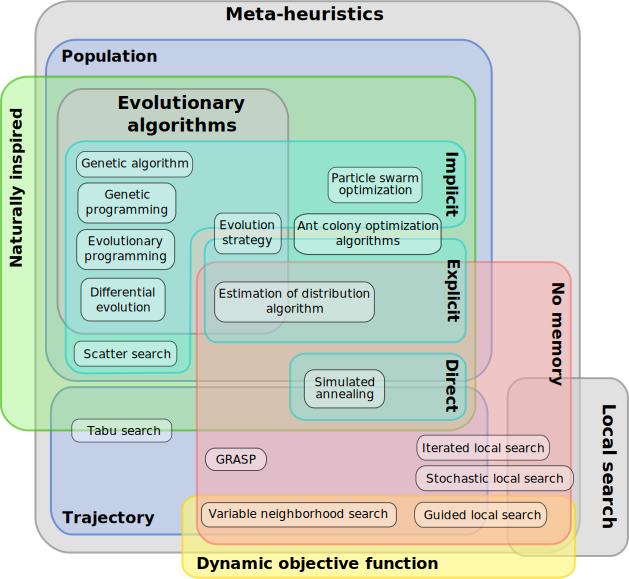
\includegraphics[width=0.7\textwidth]{graphics/Background/Metaheuristics_classification}
	\caption{Meta-heuristics Classification}
	\label{BG: MH classification}
\end{figure}


\subsubsection{Examples}\label{BG: MH Examples}
We shortly describe some prominent and widely used meta-heuristics, since later we use them as the LLH in developed Hyper-Heuristic, described in section~\ref{Impl: LLH}.


\paragraph{Evolutionary Algorithms (EAs).} Evolutionary Algorithms are directly inspired by the processes in nature, described in evolution theory. The common underlying idea in all these methods is as following. If we put a population of individuals (Solutions) into an environment with limited resources (population size limit), a competition processes cause natural selection, where only the best individuals survive (compared by the object of optimization for given subject TS )~\cite{eiben2015evolutionary}.
Tree basic actions are defined as operators of EAs: the \textit{recombination} that is applied to selected candidates Solutions (parents) among available in population to produce new ones (children); \textit{mutation} occurs in one candidate to turn it into a new Solution. Applying both operators on the parents create a set of new Solutions — the offspring, whose results evaluated using TS. After that, the \textit{selection} operator applied among available Solutions (parents and offspring) to keep the population size within defined boundaries. This process is repeatedly iterated until some termination criteria fulfilled, for instance maximal number of iteration reached, amount of TS evaluations exceed, or Solution with required quality found. The work-flow of EA depicted on picture \ref{bg:pic:EAs}.

\begin{figure}
	\centering
	\includesvg{EA}
	\caption{Evolutionary Algorithm Control Flow}
	\label{bg:pic:EAs}
\end{figure}

\paragraph{Genetic Algorithm (GA).} It is the first association coming into mind when you hear words 'Evolutionary Algorithms'. GA traditionally has a fixed work-flow: with given initial population of $\mu$ usually randomly sampled individuals, the parent selection operator shuffles initial set to create a random pairs of parents, after that the crossover operator is applied to each pair with probability $p_c$ to produce children. Then newly created Solutions individually undergoes mutation operator with independent probability $p_m$. Resulting offspring perform tournament within selection operator and $\mu$ survivals replace current population~\cite{eiben2015popular}. Distinguishable characteristics of simple GA are following: Solution representation in form of bit-strings, one-point crossover and bit-flip usage as the recombination and mutation operators respectively and a generational selection operator (survive only children).

\paragraph{Evolution Strategy (ES).} In contradiction to GA, Evolution Strategy algorithms are working in a vector space of Solution representation and distinguish $\mu$ individuals population size and $\lambda$ offspring generated in one iteration. They induce a very useful feature of \textit{self-adaptation}: changing the mutation step sizes depending on control parameters. The self-adaptive information (which is related entirely to EA, but not to OP under consideration) is appended to the individual's chromosome. While the general work-flow for all EAs remains the same, underlying operators are changed. Here, parent selection operator take a whole population into consideration, the recombination scheme could involve more than two parents to create one child. To construct a child, recombination operator adds alleles from parents in two possible ways: with \textit{uniform} probability for each parent (discrete recombination), or averaging the values of alleles (intermediate recombination). There are two general selection schemes that are used is such algorithms: $(\mu,\lambda)$ which discards all parents and selecting only among offspring highly enriching exploration, and $(\mu+\lambda)$ which includes predecessor Solutions into selection which also known as \textit{elitist selection}~\cite{eiben2015popular}.

\paragraph{Simulated Annealing (SA).} This meta-heuristic is inspired by the annealing technique used in the metallurgy to obtain 'well-ordered' solid state of metal, imposing a minimal internal energy and avoiding semi-stable structures, characterized by local energy minimums. The search process here treated as the metal with a high temperature at the beginning and lowering it to minimum while approaching the end. %SA algorithm handles the optimization objective as annealing threat the material energy. 
SA starts with initial Solution $S$ creation (randomly or using some heuristic) and temperature parameter $T$ initialization. At each iteration, new solution candidate $S^*$ selected within the neighborhood $N(S)$ of current $S$ and the selection criteria evaluated based on $S^*$ quality and temperature parameter $T$. $S^*$ replaces $S$ if (1) optimization objective $f(S^*)$ dominates over $f(S)$ or (2) with a probability that depends on quality loose and current temperature: $p(T, f(S^*), f(S)) = \exp(-\frac{f(S^*) - f(S)}{T})$ for minimization OP and $p(T, f(S^*), f(S)) = \exp(-\frac{f(S) - f(S^*)}{T})$. At each iteration the temperature parameter $T$ is decreased following \textit{Annealing Schedule} also called as \textit{Cooling Rate}: linearly, inverse logarithmic, exponentially~\cite{boussaid2013survey}. The weak side here is that the Annealing Schedule is problem dependent and cannot be determined beforehand, however SA algorithms with parameter control do exist and address this problem by changing the Cooling Rate or temperature parameter $T$ during the search process, refer~\cite{ingber2000adaptive} and~\cite{de2003placement} respectively.

\subsection{Hybrid-Heuristics}
The hybridization of different systems constantly provides a positive effect — you take advantages of one system and merge them with the strong sides from other those getting the best from both of them. The same could be applied for the heuristics. Imagine you have two algorithms biased towards exploration and exploitation respectively. If you use them separately, the expecting results in most cases may be way far from optimal as the outcome of disrupted diversification-intensification balance. But with merging them into say stages of hybrid heuristic, one will obtain both advantages of finding a good quality results and escaping local optima. Most of available hybridization are done exactly with this idea — \textit{staging combination} two heuristics, one exploration and second exploitation suited for getting outperforming hybrid.


\subsubsection{Examples}

The methods to construct hybrid mostly defined by the undertaken heuristics and those, to the best of our knowledge, could not be generalized and classified well, except a \textit{staging} approach, when the output of one algorithm is used as initial state of other, is broadly used. Instead, we will introduce some examples of performed hybridization in order to give you a better understanding of possible hook parts within algorithms and influence of aforementioned balance onto the search process.

\paragraph{Guided Local Search ($GLS$) + Fast Local Search ($FLS$) \cite{tsang1997fast}.}
It is an example of repeatedly applying two heuristics in sequence (staging) and passing the output from one to second one.
The main focus of $GLS$ here is on the Search Space exploration and process guidance using incubated information. In some sort, $GLS$ is closely related to the \textit{Frequency-based memory} used in Tabu Search. In runtime, $GLS$ modifies the cost function of the problem to include penalties and passes this modified cost function to local search procedure. The penalties form memory that describe a local optimum solution and guide the process out of it. A local search procedure then carried out by $FLS$ algorithm. The main feature of $FLS$ is the ability to quickly traverse a neighborhood. It is done by braking it into a number of small sub-neighborhoods, and ignoring those without an improving moves. By performing depth first search over these sub-neighborhoods. At some point of time $FLS$ appears in the local optimum, passes back control to $GLS$ and iteration repeats. 

\paragraph{Direct Global + Local Search \cite{syrjakow1999efficient}.}
As stated in the name this hybridization combines global and local optimization strategies into two-stages: stochastic global pre-optimization and deterministic local fine-optimization. For global optimizations authors apply one of two well-known meta-heuristics — Genetic Algorithm, or Simulated Annealing described earlier in section~\ref{BG: MH Examples} with Meta-heuristics examples. The transition from Global to Local search happens when the predefined conditions are met, for instance when the number of Target System (goal function) evaluations exceeds a boundary or when no distinguishable improvement was done. The Pattern Search~\cite{hooke1961direct} algorithm also known as direct, derivative-free, or black-box search plays role of Local Search heuristic in this combination. Hybrid-heuristic terminates when Pattern Search converges.

\paragraph{Simulated Annealing + Local Search \cite{martin1996combining}.}
After brief explanation of previous two hybrids, an observant reader might make a guess what happens in this particular case, and he will be completely right!
Authors named this method 'Chained Local Optimization', in other words it is yet another representative of staged hybridization. Iteration starts with the current Solution perturbation (authors called this action a 'kick', referring a dramatic change of current position within a Search Space). After this, the Local Search heuristic applies to intensify obtained Solution. When the local optimum reached, the control flow returned to the Simulated Annealing for acceptance criteria evaluation in order to accept or reject a new Solution, what concludes an iteration.


\paragraph{$EMILI$~\cite{pagnozzi2019automatic}} 
Easily Modifiable Iterated Local search Implementation ($EMILI$) is a framework-like system for automatic generation of new (hybrid) stochastic Local Search algorithms. $EMILI$ is a solver for Permutation Flow-Shop Problems (PFSP), also known as Flow Shop Scheduling problems which define a search of an optimal sequence of steps for product creation within a workshop.
Here authors have implemented algorithmic- and problem-specific building blocks, defined grammar-based rules for those building blocks composition and use an automatic algorithm configuration tool $IRACE$~\cite{lopez2016irace} to find a high performing algorithm configurations for problem solving. The work-flow of $EMILI$ could be described in three steps: (1) adaptation of rules to specific representations type of PFSP problem objectives (either Makespan, Sum completion times, Total tardiness), (2) generate a set of possible hybrid heuristics for each of PFSP type and (3) apply iterated racing algorithm implemented in $IRACE$ to select the best performing hybrid for specific problem type. 

From our perspective, described approach of automatic algorithm generation is very close to construction Hyper-Heuristics strategies with off-line learning described in section~\ref{bg: hh}, however authorized to change the system class (from hybrid- to hyper-heuristic) defined by $EMILI$ authors.


\subsection{No Free Lunch Theorem}
A nature question could arise ``If we have all this fancy and well-performing heuristics, why should we spend effort and develop new algorithms, instead of using existing?'' And the answer to this question is quite simple — the perfect algorithm suited for all OP that will do not exist and can not exist. All algorithms that search for optimal parameters of a Target System perform exactly the same, when the results are averaged over all possible Target Systems. If an algorithm is gaining the performance in one problems class, it loses in another class. This is a consequence of so-called \textbf{No Free Lunch Theorem} (NFLT)~\cite{wolpert1997no}.

In fact, one could not predict, how exactly will behave one or another algorithm with problem in hand. A possible and the most obvious way is to probe the specific approach, and analyze it behavior with respect to another in problem solving process. Here simple heuristics and meta-heuristics are out of competition, since if you solved the Optimization Problem once, you wouldn't optimize a second time.
Here come \textbf{Hyper-Heuristics}. We will proceed with their description and how they deal with the NFLT consequences in following section, to not switch the thesis.


\subsection{Hyper-Heuristics}\label{bg: hh}
Lots of state-of-art heuristics and meta-heuristics are developed in a very domain-dependent way, say they use the domain knowledge too intensively to be broadly reused. It motivated research community to raise the level of generality at which the optimization systems can operate and still provide good quality Solutions for various Optimization Problems. The term \textbf{Hyper-Heuristic} (HH) was defined to describe an approach of using some High-Level-(Meta-)Heuristics (HLH) to choose other Low-Level-(Meta-)Heuristics (LLH) and use it to solve the OP in hand. Indeed, a combination of different low-level heuristics produced better results than if hey were applied separately~\cite{drake2019recent}.
It can be explained by the nature of search process and how it evolves in time. When you apply heuristic, it sooner or later converge to some extreme point, hopefully global optimum, since it is `blind' to those not visited regions in the Search Space. But changing the trajectory of investigation by (1) drastically varying the Neighborhood, (2) changing the strategy of Neighborhood exploration and exploitation could (1) bring you to those previously unreachable zones (2) rapidly. However, it is not possible to predict how one LLH will behave in every stage of the search process in comparison to another, here HLH comes to help. In \cite{moriarty1999evolutionary} authors made infer that Hyper-Heuristics can be viewed as a form of Reinforcement Learning, which is sounds logically.

\begin{figure}
	\centering
	\includesvg{HH}
	\caption[Hyper-Heuristics]{Hyper-Heuristics\protect\footnote{Icons from \href{https://thenounproject.com/}{thenounproject.com}}}
	\label{bg:pic:HH}
\end{figure}

%\footnotetext[1]{Icons from \href{https://thenounproject.com/}{thenounproject.com}}


The new concept which implicitly was used in Meta-Heuristics, but explicitly pointed out in Hyper-Heuristics is the \textbf{Domain Barrier}.
As we told previously, HH do not directly tackle an OP, they use LLH instead. This means, that HH are usually unaware of the domain details such as what are those data types, their relationship, etc. within a domain, but rather encapsulates this information in LLHs and those could be used to broader range of Optimization Problems as it is illustrated on picture~\ref{bg:pic:HH}.


\subsubsection{Classification}
Although, the research in Hyper-Heuristics field actively ongoing, a lot of different instances were already created and some trials to organize approaches were conducted~\cite{ryser2014review,drake2019recent,burke2019classification}.
Researchers in their surveys classify HHs by different characteristics, some of them overlap, but it also happens that intriguing parameters distinguished were not highlighted in other works. 

In this section we present some (but not all) facets of Hyper-Heuristics classification to better justify the goal of this thesis.


We begin with the two broadest classes, which differentiate HH \textit{routine} or also called as \textit{nature of High-Level-Heuristic Search Space}~\cite{burke2013hyper,burke2019classification,drake2019recent}.
The first class is the Hyper-Heuristics to \textbf{select} Low-Level-Heuristic, in other words \textbf{Selection Hyper-Heuristic}. In previous sections we were implicitly referring to this class, while talking about Hyper-Heuristic approaches in general. These algorithms operate in the Search Space defined by simple Low-Level-Heuristics that solve Optimization Problem. The task of HLH is to pick the best suited LLH based on available prior knowledge and apply it to OP underway.
The second class is the Hyper-Heuristics to \textbf{construct} or generate LLH by using the atomic components of other heuristics as Lego bricks and following some predefined receipt. These approaches could lead to creating new and unforeseen heuristics that are expected to reveal good performance~\cite{burke2019classification} while solving the problem in hand.


Next, the distinction in \textit{nature of Low-Level-Heuristics Search Space}, in other words how do the LLH derive Solutions for the OP in hand~\cite{burke2013hyper,burke2019classification,drake2019recent}, either by \textbf{constructing} a Solution each time from scratch, or by \textbf{perturbation} of already existing one.


The other broadly used characteristic is the \textit{use of memory}. From this perspective we distinguish Hyper-Heuristics in which the learning happens on-line, off-line or learning mechanisms are not present at all~\cite{ryser2014review,burke2019classification}.
\begin{itemize}
	\item In \textbf{on-line} case, the HH derives an information, used to select among LLH, while those LLH are solving a problem.

	\item In \textbf{off-line} case, the learning happens before solving an Optimization Problem. Here one should first train an HH using other, but homogeneous to current problems. After this preparation step, the HH could be applied to problem in hand.

	\item There exist also \textbf{mixed} cases, where learning happens both on-line and off-line. Definitely it is a promising research direction, despite high dependency on off-line phase.
	
	\item The last case here is an approach \textbf{without learning} mechanisms involved. Usually, these Hyper-Heuristics perform some sort of Random Search selection of LLH.
\end{itemize}


Yet another faced of Hyper-Heuristics classification is the way of assigning \textit{hyper-parameters} (here we use parameters and hyper-parameter concepts interchangeably) for LLHs, or their components~\cite{drake2019recent}. We analyzed surveys and find out that some researchers do not explicitly differentiate approches with respect to nature of parameter settings~\cite{ryser2014review,burke2013hyper,burke2019classification}, while other do~\cite{drake2019recent}:
\begin{itemize}
	\item In \textbf{static} assignment, the underlying heuristics use provided beforehand (usually default) hyper-parameters and do not change them while solving the problem in hand.

	\item The \textbf{dynamic} case uses some kind of rule for parameters changing, specified in advance.

	\item There exist also an \textbf{adaptive} approach, in which HH assigns the parameters for LLH as the response to the learning process. In some sort, it is similar to the parameter control techniques used in Meta-heuristics.
	
	\item And finally, a \textbf{self-adaptive} approach where underlying LLHs comprise \textit{parameter control} techniques and those search for the best solution for OP and own parameter settings simultaneously.
\end{itemize}


For more detailed analysis, description, other classification facets and respective Hyper-Heuristic examples we encourage reader to look into~\cite{burke2003hyper,ryser2014review,drake2019recent,burke2019classification} researches.

\subsubsection{Examples}\label{bg: hh examples}% should I present it in following sections?
\paragraph{HyFlex~\cite{ochoa2012hyflex}}\textit{Hyper-Heuristics Flexible Framework}. It is a software skeleton, created specifically to encourage researchers creating Hyper-Heuristics. It provides the implementation of components for 6 problem domains (Boolean Satisfiability, Bin Packing, Personnel Scheduling, Permutation Flow Shop, Traveling Salesman and Vehicle Routing problems), evaluation functions and a set of Low-Level-Heuristics. The benchmark sets as well as comparison to other existing HH is included to framework. The intent of $HyFlex$ creators to provide these features was to enable others focus directly on High-Level-Heuristics implementation without need to challenge other minor needs and those bring clear comparison among HLH performance~\cite{ochoa2012hyflex}. From the classification perspective, all derivatives from the $HyFlex$ framework are Selection Hyper-Heuristics, however they utilize different learning approaches and hyper-parameter settings. Algorithms, built on top of $HyFlex$ framework could be found in~\cite{misir2012intelligent,ryser2014review,drake2019recent} or on the CHeSC 2011 challenge website\footnote{\href{http://www.asap.cs.nott.ac.uk/external/chesc2011/}{Cross Domain Heuristic Search Challenge website: asap.cs.nott.ac.uk/external/chesc2011/}}.


Along with $HyFlex$, a number of Hyper-Heuristic frameworks is growing, some of them are under active development while others are abandoned:
\begin{itemize}
	\item $Hyperion$~\cite{swan2011hyperion} is a $TH$ (recursive template and hook) framework aiming to extract information from OP search domain for identification of promising components.
	
	\item $hMod$~\cite{urra2013hMod} framework allows not only to construct algorithm components using predefined abstractions (such as $IterativeHeuristic$). In current development stage, developers of $hMod$ are focusing on creation of mechanisms rather than providing a set pre-built heuristics. 
	
	\item $EvoHyp$~\cite{pillay2017evohyp} focus on hyper-heuristics with evolutionary algorithms used as Low-Level-Heuritics. Here authors enable users of framework to construct both selection and generation HHs for both types construction and perturbation LLHs.
	
\end{itemize} 

\paragraph{HITO~\cite{guizzo2015hyper}}\textit{Hyper-Heuristic for Integration and Test Order Problem}. It is an example of HH for selection of LLH. LLHs in this case are presented as a composition of basic EAs operators — crossover and mutation forming multi objective evolutionary algorithms (MOEA). HH  selects those components from $jMetal$ framework\cite{durillo2011jmetal} using interchangeably Choice Function (in form of weighted linear equation) and Multi Armed Bandit based logic to yet again balance exploitation of good LLHs and exploration of new LLHs.


\paragraph{MCHH~\cite{mcclymont2011markov}}\textit{Markov Chain Hyper-Heuristic} is an on-line selective Hyper-Heuristic for multi-objective continuous problems. It utilizes reinforcement learning techniques and Markov Chain approximations to provide adaptive Heuristic selection method. While solving an OP, $MCHH$ updates prior knowledge about the probability of producing Pareto dominating Solutions by each LLH using Markov Chains those guiding an LLH selection process. Applying on-line reinforcement learning techniques, this HH adapts transition weights in the Markov Chains constructed from all available LLHs those updating prior knowledge for LLH selection.


\subsection{Conclusion on Heuristic Solvers}
To conclude our review on Heuristic approaches for Optimization Problems solving, we shortly remind you pros and cons of each heuristic level.

On the basis remain Simple Heuristics with all their domain-specific knowledge usage and particular tricks for solving problem in hand. Usually, they are created to tackle a concrete problem in hand applying simple algorithmic approach. The simplicity of application and usually fast runtime is balanced by medium solution quality.

On the next level inhabit Meta-Heuristics. They could be compared with more sophisticated hunters which could not only charge directly, but also take a step back when stuck in a dead end. This additional skill enables them to survive in a new environment (Optimization Problem), however some adaptations should be performed to understand the problem and parameter tuning to perform well.

Among with MHs, Hybrid-Heuristics do exist. It is nothing special here, they just took some survival abilities from several Meta-Heuristics hoping to outperform, however still requiring adaptation. In some cases this hybridization provides it advantage, but as time shows, they did not kick out MHs and reside together with their parents. Those we can conclude that the exposed balance between development effort and providing results quality not always assure users to apply them.

Finally, the chosen ones that lead the others, Hyper-Heuristics are inhabitants of the upper level generality. 
Operating by the other Heuristics, HHs analyze how good former are and definitely make use of this knowledge by solving concrete problem using the best suited Heuristic.
Imposing such great abilities, Hyper-Heuristics are able to tackle not only the concrete optimization problem, but entire class of problems, although requiring more development effort.


\section{Parameter Tuning as an Optimization Problem}\label{bg: parameter tuning}
Most of existing learning algorithms expose some parameter set, needed to be assigned before applying this algorithm to solve a problem. Modifying these parameters, one could change the system behavior and possible result.

When we are talking about parameter tuning problem, the following terms should be refined explicitly:
\begin{enumerate}
	\item \textbf{Target System (TS)} is the subject of parameter tuning optimization problem. Simply, it is the system which parameters are tuned.
	\item \textbf{Parameter} a.k.a. Hyper-Parameter (HP) is one of exposed by TS hooks for tuning. Should be described in terms of type and possible values.
	\item \textbf{Configuration} is formed by unique combination of parameter values, required to run TS.
	\item \textbf{Search Space} is formed by all possible Configurations for defined HPs.
\end{enumerate}

In \textit{machine learning} these parameters are called \textbf{Hyper-Parameters}. Note, that we are referring both terms $Parameters$ and $Hyper-Parameters$ $(HPs)$ interchangeably through the thesis.


For instance, consider neuron network. Hyper-parameters in this case will specify the structure (number of hidden layers, units, etc.) and learning process (learning rate, regularization parameters, etc.) of network. Changing them will result in changes of system accuracy.


One of the most frequent optimization applications is \textbf{Parameter Tuning} — searching of hyper-parameter values to optimize some characteristic of system. When talking about our example, we could apply Parameter Tuning to maximize network accuracy. Considering simultaneously number of characteristics such as running time + accuracy results in Multi-Objective Parameter Tuning.
When talking about heuristics, proper assignment of hyper-parameters has a great impact on exploration-exploitation balance and those on algorithm performance.


% the motivation of using parameter tuning system as basis for hyper-heuristics
We believe, that a central role of off-line selective Hyper-Heuristics, namely solving the algorithm selection problem could be represented as the parameter tuning problem, where instead of parameter selection we select entire system according to reported performance. With this idea in mind, we investigate a possibility of turning parameter tuning system into a Hyper-Heuristic.
For doing so, our next step is the review and comparison of existing parameter tuning approaches and systems. 


\subsection{Approaches for Parameter Tuning}
Nowadays there exist wast number of ways to assign parameters for system. 
One of the simplest and error-prone ways is just trusting your (or someones else) intuition and using those parameters that seems to you more or less logic for particular system and problem instance. People quickly abandoned it in favor of automatic approaches, since novel computational capacities easily provide a possibility for it.

We briefly outline existing automated approaches illustrating each with a picture~\ref{bg: fig:automated parameter tuning approaches}. Each graphic shows dependencies between parameters $X_1$ ($x$ axis), $X_2$ ($y$ axis) and optimization subject values (which we are maximizing here) along those axes.

\begin{figure}
	 \centering
	\begin{subfigure}[b]{0.25\linewidth}
		\includegraphics[width=\linewidth]{graphics/Background/hyperparameter-grid-search.png}
		\caption{Grid Search.}
		\label{bg: fig:automated parameter tuning approaches: grid}
	\end{subfigure}
	\begin{subfigure}[b]{0.25\linewidth}
		\includegraphics[width=\linewidth]{graphics/Background/hyperparameter-random-search.png}
		\caption{Random Search.}
		\label{bg: fig:automated parameter tuning approaches: random}
	\end{subfigure}
	\begin{subfigure}[b]{0.25\linewidth}
		\includegraphics[width=\linewidth]{graphics/Background/hyperparameter-learning-search.png}
		\caption{Learning Search.}
		\label{bg: fig:automated parameter tuning approaches: learning}
	\end{subfigure}
	\caption{Automated Parameter Tuning Approaches\protect\footnote{Graphics from~\cite{koch2017automated}}.}
	\label{bg: fig:automated parameter tuning approaches}
\end{figure}


\paragraph{Grid Search.} It is a simple approach of solving the search problem by exchanging enumeration of possible solutions (parameter sets) for relaxed problem instance. This relaxation is derived by user specifying finite number of possible values for each of hyper-parameters under consideration. After evaluating each possible configuration for system under estimation, algorithm reports the best found solution. Obviously, this approach could skip promising parts of search space as shown on picture~\ref{bg: fig:automated parameter tuning approaches: grid}.


\paragraph{Random Search.} This methodology relies on random (usually uniform) sampling of hyper-parameters and their evaluation on each iteration. At first sight, it might look unreliable to chaotically traverse the search space. But empirical studies show that with growing number of evaluations this technique starts to outperform grid search~\cite{bergstra2012random}. Compare visually the best configurations (highlighted in pink) found by grid (picture~\ref{bg: fig:automated parameter tuning approaches: grid}) and random search (picture~\ref{bg: fig:automated parameter tuning approaches: random}) techniques.

\paragraph{Model Based Search.} In most cases, the dependencies between tuned parameter values and optimization objective do exist, can be observed and utilized for hyper-parameter tuning by predicting which parameter combinations could produce a better results, those making guesses more precise. As it showed on picture~\ref{bg: fig:automated parameter tuning approaches: learning}, after accumulating more information, learning algorithm will make more precise guesses, what in contrast to previously described model-free approaches is more preferable and robust.
With this idea researchers started to build systems that (1) traverse the search space more efficiently and (2) could mimic dependencies between parameters and objective resulting in surrogate models. The later is some sort of enhancement used in combination with former enabling you to simulate evaluation of real system instead of expensive real probe.



\subsection{Systems for Model-Based Parameter Tuning}\label{bg: parameter tuning expamples}
The parameter tuning is an obligatory task for getting the maximum system performance and should be done at design time.
Novel approaches for tuning are usually built in form of frameworks with exposed hooks for attaching system under estimation.

Naturally, the Target System evaluations here supposed to be extremely costly since they require real execution of target algorithm, that is why algorithms in those frameworks are trying to utilize every single bit of information from evaluations, building surrogate models and using Bayesian optimization approaches for making each evaluation valuable.

In this section we review some among existing open-source parameter tuning systems from following perspectives:%, that could be used as basis for Hyper-Heuristic.
%TODO: in implementation. While analyzing, we discuss each system with following perspectives, highlight characteristics that later will be used to select the best suited system as basis for Hyper-Heuristic:
\begin{itemize}
	\item \textbf{Conditional parameters support} It exposed for user ability of tuning system to describe and tackle conditional dependencies between hyper-parameters. As an example imagine parameter that can take only some specific values, for instance \textit{crossover type} in Genetic Algorithm could be \textit{Partially Mapped Crossover ($PMX$)}, \textit{Cycle Crossover ($CX$)}, etc.~\cite{larranaga1999genetic} Selecting concrete crossover type, one will also need to specify respective parameters for this crossover type. But it could turn out, that these parameters are illegal, when the other crossover type is selected. This type of dependency could be described by parent-child relationship, however other types of dependencies also exists.
	
	\item \textbf{Parameter types support} It is one of basic features required in system to be usable. Namely, Target System parameters could be not only numerical (more concretely integer or fractional), but also categorical in form of strings, boolean values, etc. Considering categorical data types, they could be either nominal or ordinal. Difference between categorical types lays in fact, that the latest depict not only possible atomic values, but also order between them. For concrete example we discuss the Genetic Algorithm again with following parameters: population size (numerical integer in range $[1...\inf)$), mutation probability (numerical fractional $[0...1]$), crossover type (categorical nominal ${PMX, CX}$). Indeed, population size could also be displayed as a set of finite values ${10, 100, 1000}$ (categorical ordinal type).
	
	\item \textbf{Extensibility} This feature is crucial in cases, if one would like to try a new promising and intriguing learning algorithm, that was not included in parameter tuning system yet. In fact, one may need not only new learning algorithm, but other features like non-trivial stopping criterion, tools for handling stochastic behaviors, or different strategies for random sampling (which are utilized while tuning system is learning before making a prediction).
	
	\item \textbf{Parallel Evaluations }The simultaneous evaluation of multiple Configurations required for utilizing available computing resources that could scale horizontally. 
	
	% TODO: implementation \item[Support for Online Problem Solving.] This is a bit complex characteristic of system that we are willing to distinguish. As it turns out, most parameter tuning systems require full evaluation of Target System for Configuration comparison. However, in case of Hyper-Heuristic, the Configuration evaluation is a trial to solve the problem in hand using particular $LLH$ (tuned parameter) Here we compare final result quality, reported by each $LLH$
	
\end{itemize}


\subsubsection{IRACE~\cite{lopez2016irace}}\label{bg: irace}
The first system under investigation is an implementation if Iterated Racing Algorithm\cite{birattari2010f} in \textbf{IRACE} package for off-line hyper-parameters tuning.
The underlying methodology consists three main steps: (1) using prior knowledge, sample new Configurations, (2) distinguish the best ones among sampled using racing algorithm and (3) update prior knowledge to bias next samplings in (1) towards better Configurations. 
Prior knowledge here represented as probability distribution for each tuned parameter independently (truncated normal and discrete distributions for numeric and categorical hyper-parameters respectively). During update step (3), the probability distributions are increased for those values, where the best Configurations were found.

Racing step (2) could be described as process of running Target System using Configuration under evaluation on a set of heterogeneous problem instances. While solving those instances, the statistically worse-performing Configurations are rejected and racing proceeds with remaining ones. This process continues until reaching required number of survivals or number of solved problem instances. 

As it was mentioned above, \textbf{IRACE} supports various data types such as numerical and categorical as well as the possibility of conditions description. While the problem of data types solved by different distributions used, the conditional relationships are determined by the dependency graphs. During sampling (1), first non-conditional and only afterwards dependent parameters are sampled, if respective conditions are satisfied. The framework highly utilize racing algorithm for evaluations and \textit{Friedman test}~\cite{conover1980practical} or alternatively \textit{paired t-test} for statistical analysis of parameters, those it is static in terms of variability and extensibility of learning mechanisms. In terms of parallel evaluations, the algorithm is doing well at the beginning of each racing step, however as the process proceeds less and less evaluations are executed in parallel those all available resources are utilized optimally at all steps of algorithm.


\subsubsection{SMACv3~\cite{hutter2011sequential}}\label{bg: smac}
Sequential Model-based Algorithm Configuration (\textbf{SMAC}) is a system for parameters optimization developed by AutoML research group (here we review \textbf{SMACv3}). 

In this research, scientists generalized the process of parameter tuning under the term \textit{Sequential Model-Based Optimization (SMBO)} as iterations between fitting models and using them to make choices of Configurations.

It is an extension introducing learning models to previously existing Random Online Aggressive Racing (\textbf{ROAR}) mechanism. Authors in their research showed that the machine learning mechanisms and regression models in particular could be applied not only for tuning parameters, but also for optimizing any expensive black-box functions in general (we believe that the last holds also for the majority of other parameter tuning systems). 

This system development was directed to tackle existing (at that point of time) limitations of all published \textbf{SMBO} approaches, namely expanding an applicability not only to numerical, but also to categorical parameters and optimizing target algorithm not only on single, but on number of problem instances (benchmark set of problem instances) for facing the variance.
A routine in Sequential Model-based Optimization is somehow similar to one implemented in \textbf{IRACE} and could be imagined as iterated application two tree steps: (1) building learning model, (2) using it for making choices which Configurations to investigate next and (3) actual evaluation of sampled Configurations.
The evaluation (3) here carried out by original ROAR mechanism in which evaluation of each new candidate Solution continues until enough data (from benchmark set of problem instances) obtained to either replace current Solution or reject candidate. In contrary to original model-less ROAR, at step (1) \textbf{SMAC} builds machine learning regression random forest~\cite{breiman2001random}. The usage of regression decision trees (which form the forest) was motivated by known fact that they are known to fit well with categorical data. Later, at step (2) an Iterative Local Search (\textbf{ILS}) heuristic applied in combination with Bayesian optimization technique evaluating \textit{Expected Improvement} (EI). \textbf{ILS} started on the best previously found Configurations and was used for sampling new promising ones while distinguish between them carried out by EI using regression model built at step (1). EI is large for those Configurations, with low predicted cost, or for those with high uncertainty those providing exploration-exploitation balance automatically~\cite{jones1998efficient}.

% TODO: try a random forest as a 1ST level of HH, SMAC paper (short version), PAGE 7, CITES 18, 19.

Exposing such a great learning capabilities and using Expected Improvement technique that guarantees to converge the search process to global optimum given enough time, the major drawback in this system is lack of flexibility to include conditional dependencies between parameters into search space description. 
One of possible solutions here could be the use of conditional-aware neighborhood definition in \textbf{ILS} (currently it just carried out by sampling in Gaussian distribution). In fact, used Search Space representation framework ConfigSpace\cite{configspace} is able to specify dependencies among hyper-parameters and verify the Configuration validity in terms of parameter conditions violation. However, to the best of our knowledge, during the Configuration sampling those conditions are not taken into account and could be broken thus resulting in illegal parameter combination. Obviously those cases are handled and broken Configurations are rejected, but in case of `sparse' Search Spaces (where significant amount of parameter combinations are restricted by conditions) this approach could lead to ineffective sampling and predictive abilities of system will suffer greatly. Unfortunately, we did not find any officially published evaluations of such cases and could only make guesses based on own intuition and framework developers advises for SMACv3 application in such cases~\footnote{Visit GitHub repository of SMACv3 for more info~\url{https://github.com/automl/SMAC3/issues/403}}.

ROAR mechanism is the derivative from \textbf{FocusedILS} algorithm (solver in \textbf{ParamILS} parameter tuning framework~\cite{hutter2009paramils}) where each evaluation of new candidate Solution on problem instance performed sequentially. Since the ROAR evaluation strategy is applied at step (3), we conclude that the utilization of, in principle, available parallel computation capabilities is another drawback of \textbf{SMACv3} framework.


\subsubsection{BOHB~\cite{falkner2018bohb}}\label{bg: bohb}
While SMAC outperforms and partially reuses decisions done in ParamILS, BOHB (Bayesian Optimization combined with HyperBand) is the parameter tuning tool that outperforms SMAC and was introduced by the same AutoML research group.

As it stated in name, the main routines here are carried out with mainly two algorithms: learning (1) and Configurations sampling (2) is done with Bayesian Optimization technique Tree Parzen Estimator (TPE) while Configurations evaluation and comparison carried out by HyperBand (HB) algorithm.

The TPE instead of na\"ive Gaussian Processes-based (GP BO) Bayesian Optimization was motivated by better dimensional scaling and internal support of both numerical and categorical data types (however, some minor transformations are still required). Unlike GP where optimization done by modeling distributions of Configuration results given it parameters, TPE builds two \textit{parameter distributions} splitting Configurations into two sets according to their `goodness'. For more detailed explanation we refer to original TPE description~\cite{bergstra2011algorithms}.

The other part of BOHB, namely HyperBand is a promising multi-armed bandit strategy for hyper-parameter optimization~\cite{li2017hyperband} in which the \textit{budget} for Configurations evaluation is defined beforehand and divided into iterations. The role of budget could play any control parameter that denotes the accuracy of Configuration evaluation by TS where the maximum budget gives you the most precise Configuration evaluation while minimum amount results in the least accurate approximation of result.
Running examples of budget could be the number of iterations in iterative algorithm or time to train the neuron network.
As the result, requirements arise for TS to expose and support budget usage as expected in algorithm.
At each iteration, HB randomly samples a number of Configurations for evaluation which, in fact, decreases for former iterations while the amount of budget remains the same. As the outcome, first iterations of HB are full of coarse-grain evaluated Configurations while later iterations produce higher number of more accurate measurements. At each iteration of HB, the Successful Halving (SH) procedure is executed to drop (usually $\frac{2}{3}$) badly performing Configurations. As one could expect, since the number of measuring Configurations in each iteration decreases, the measurements could be done more precisely since the amount of SHs execution drops too.

Binding of HyperBand and Bayesian Tree Parzen Estimator exists is several places. Firstly, the learning models are updated each time when new results are available for every budget value. Next, at each iteration of HB, TPE model is used for sampling new Configurations. Note that BOHB uses model built with results obtained with the largest budget only. This decision leads in more precise predictions in the later stages of parameter optimization procedure.

The drawback of this system lays in the way of handling conditions between hyper-parameters. BOHB actual implementation HpBandSter (a distributed HyperBand implementation on Steroids)~\footnote{GitHub repository: \url{https://github.com/automl/HpBandSter}} as SMACv3 system uses ConfigSpace framework for Configuration Space definition. As we discussed in SMACv3 description (section~\ref{bg: smac}), it naturally allows to encode the dependencies and conditions among parameters within space. As authors stated, the TPE learning models accomplish this knowledge implicitly by shrinking the densities for forbidden parameters (actually those parameters are still added to models by \textit{imputation} mechanism where empty or default values are assigned). 
However, consider case of two Configurations $C_1$, $C_2$ appearance such that some parameter $P_i$ is forbidden in $C_1$, but not in $C_2$. The actual number of such parameters could vary dramatically in `sparse' Search Spaces those distributions estimated by KDEs will not reflect the reality. As a consequence, the prediction performed using such distributions will often result in `invalid' Configuration within `sparse' spaces hurting the performance and accuracy of sampling.

% TODO: it is more for concept description
% Even if fix of Configuration sampling in such cases is relatively simple task (parent-child relationship utilized in IRACE), then building proper density distributions of `good' parameters reflecting conditions is hard.


\subsubsection{Auto-sklearn~\cite{feurer2015efficient}}
From perspective of Optimization Problem solving, goals of automatic machine learning are quite similar to persecuted by Hyper-Heuristics. 
They both operate on Search Space of algorithms (or their building blocks) which later are combined and applied to problem in hand with objective to find the best performing one. In particular, based on Scikit-learn framework~\cite{scikit-learn}, Auto-sklearn system operates over number of classifiers, data and features preprocessing methods including their hyper-parameters to learn the dependencies among data and solve the classification task. %which in some sort is similar to usage of LLHs to process a Search Space.

This \textit{Combined Algorithm Selection and Hyper-parameter tuning problem} was formalized as \textit{CASH} and presented previously in Auto-WEKA~\cite{thornton2013auto} system.

The crucial decisions made in Auto-sklearn resulting into state-of-art performance and classification accuracies is the combination of off-line and on-line learning.

During the off-line phase, namely \textit{metal-learning}, researchers conducted meta-features for datasets published by OpenML community~\cite{OpenMLPython2019}. 
The entropy of results, data skewness, number of features and their classes is a sparse set of meta-features examples used to characterize a dataset (overall number is 38). After that, for each of available in meta-learning dataset, the search of best performing machine-learning pipeline was done using Bayesian Optimization technique implemented in discussed previously SMAC~\cite{hutter2011sequential} framework. The resulting combination of dataset, machine learning pipeline and its accuracy were stored and later used to seed the same Bayesian Optimization for on-line phase of pipeline search. 

During the on-line phase, the other crucial improvement was introduced. Usually, while searching the best-performing pipeline each new (except final) instance was built, trained, evaluated, results are stored, but the pipeline itself discarded. Here, the idea lays in storing previously instantiated and trained pipelines obtained while solving the CASH problem. Later they are used to form an ensemble of models and make final classification together. This mean, that the derivative of this architecture search is a set of models with different hyper-parameters and preprocessing techniques, starting from the worst performing ones (obtained at the beginning) and ending by the best suited for dataset in hand. 
Information from the meta-learning phase is used as follows: for a given new dataset they derive meta-features and select some portion of created during meta-learning pipelines that are the nearest in terms of meta-feature space. Then these pipelines were evaluated on a new dataset to form initial Configurations for Bayesian Optimization in SMAC.

However, the potential of this meta-learning approach is derived entirely from such dataset repository existence and depends on homogeneous datasets availability, while the strength of proposed on-line methodology is more universal and lays only on the applicability of underlying machine learning models and strength of optimization mechanisms.
The investigation of proposed approach universality would be rather intriguing, since Auto-sklearn was applied only to classification, but not a regression problems~\cite{feurer2015efficient,biedenkapp-ecai20}.

Field of automated machine learning is one of trending research directions those there exist many open-source (\textit{Auto-Weka}~\cite{thornton2013auto}, \textit{Hyperopt-Sklearn}~\cite{komer2014hyperopt}, \textit{Auto-Sklearn}~\cite{feurer2015efficient}, \textit{TPOT}~\cite{olson2019tpot}, \textit{Auto-Keras}~\cite{jin2019auto}, etc.) as well as commercial (\textit{RappidMiner.com}, \textit{DataRobot.com}, Microsoft’s \textit{Azure Machine Learning}, Google’s \textit{Cloud AutoML}, and Amazon's \textit{Machine Learning on AWS}) auto-ml systems.

%\paragraph{CASH, Architecture Search, } add a paragraph here, or write additional chapter? 

\subsubsection{BRISEv2}
\paragraph{approach description}
\todoy{Other systems?}


\section{Parameter control as an Optimization Problem}\label{bg: parameter control}
\subsection{Parameter Control Definition}
\subsection{Examples and Reported Impact}
impact of parameter control based on other's evaluation


\section{Conclusion}

%TODO: need to add a review of available techniques for making a predictions within conditional search spaces
% https://www.etsmtl.ca/Unites-de-recherche/LIVIA/Recherche-et-innovation/Publications/Publications-2017/Levesque_ijcnn_2017.pdf
% https://arxiv.org/pdf/1909.13404.pdf - omg, 30.09.2019 -_-, smth really similar to proposed here approach..

% remind a problem we want to solve, chosen solver, it's problems, solutions (selecting, tuning) weaknesses of approach to tackle later problem and propose own clearly outlining what we want to improve in later to tacke former.

It could be compared with a warp-engine usage on a spacecraft, which gives the possibility to travel faster than speed of light by orders of magnitude. It is definitely fast enough, however if you consider a space-folding engine for instant traveling and use it to jump onto a huge distance, while warp-engine is 


The meta-heuristic systems designers reported positive impact of parameter control embedding. 
However, as the outcome of the no-free-lunch theorem, those systems can not tolerate broad range of problems, for instance, problem classes.
In other hand, hyper-heuristics are designed with an aim to select the low level heuristics and those propose a possible solution of problem, stated in no-free-lunch theorem, but the lack of parameter control could dramatically decrease the performance of LLH (probably, I need to find a prove of this, or rephrase).

\paragraph{Scope of thesis defined.} In this thesis we try to achieve the best of both worlds applying the best fitting LLH and tuning it's parameters while solving the problem on-line.